
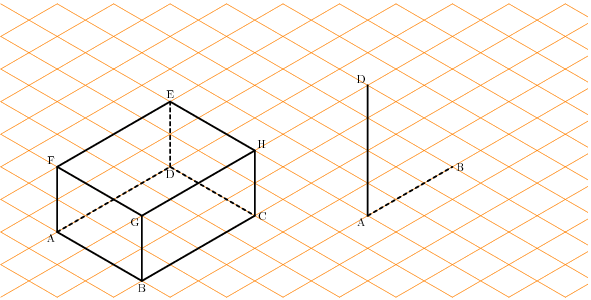
\includegraphics[scale=1]{RepS-37.png} 
\begin{enumerate}
\item Termine la représentation du pavé \ding{173}.
\item Sur le pavé \ding{172}, place un point $M$ sur l'arête
  $[BC]$ puis trace et colorie la section de ce pavé droit par le
  plan parallèle à la face $ABGF$ et passant par $M$.
\item Sur le pavé \ding{173}, place un point $I$ sur l'arête
  $[DC]$ et un point $J$ sur l'arête $[CH]$.\\Ensuite, trace et
  colorie la section de ce pavé droit par le plan parallèle à
  l'arête $[EF]$ et passant par les points $I$ et $J$.
\end{enumerate}

